\chapter{Derivatives and Gradients}
\label{chap:ch02}

% Chapter goal: the derivative as the local slope of a function, the tool
% that tells a learning algorithm which way to move each parameter.

\section{Derivatives of Functions of One Variable}
\label{sec:ch02-single}

Training a model means adjusting its parameters to make a loss smaller.
To do that, we need to know, for each parameter, whether nudging it up
makes the loss go up or down, and by how much. For a function of one
variable, that information is a single number: the \emph{derivative}.

\subsection{Slope and Rate of Change}
\label{sec:ch02-slope}

For a straight line $f(x) = ax + b$, the slope $a$ tells us how fast $f$
changes: moving the input by $h$ changes the output by exactly $ah$. Curves
have no single slope, but we can measure the average slope between two
nearby points. Between $x$ and $x + h$, it is
\[
  \frac{f(x + h) - f(x)}{h},
\]
the slope of the \emph{secant line} through $(x, f(x))$ and
$(x + h, f(x + h))$. As $h$ shrinks, the second point slides toward the
first, and the secant settles into the line that just touches the curve at
$x$ (\Cref{fig:ch02-secant}).

\begin{definition}[Derivative]
  \label{def:derivative}
  The \emph{derivative} of $f$ at $x$ is
  \[
    f'(x) = \lim_{h \to 0} \frac{f(x + h) - f(x)}{h},
  \]
  provided the limit exists. When it does, $f$ is \emph{differentiable}
  at $x$. We also write $f'(x)$ as $\dfrac{df}{dx}$ or
  $\dfrac{d}{dx} f(x)$.
\end{definition}

The derivative is itself a function of $x$: at each input it reports the
slope of the graph there. A positive derivative means $f$ is increasing at
that point, a negative one means it is decreasing, and a derivative of
zero means the graph is momentarily flat.

\begin{example}
  \label{ex:ch02-square}
  Let $f(x) = x^2$. Then
  \[
    \frac{f(x + h) - f(x)}{h}
    = \frac{x^2 + 2xh + h^2 - x^2}{h}
    = 2x + h,
  \]
  which approaches $2x$ as $h \to 0$. So $f'(x) = 2x$. At $x = 3$, the
  secant slopes for $h = 1, 0.1, 0.01, 0.001$ are $7$, $6.1$, $6.01$, and
  $6.001$, closing in on $f'(3) = 6$.
\end{example}

\begin{figure}[ht]
  \centering
  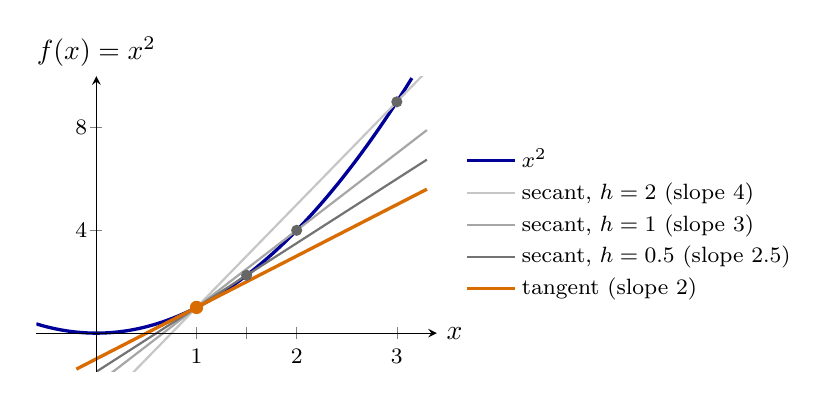
\begin{tikzpicture}
    \begin{axis}[
      width=0.55\textwidth, height=0.44\textwidth,
      axis lines=middle, axis on top,
      xmin=-0.6, xmax=3.4, ymin=-1.5, ymax=10,
      xtick={1,1.5,2,3}, xticklabels={$1$, , $2$, $3$}, ytick={4,8},
      xlabel={$x$}, ylabel={$f(x) = x^2$},
      x label style={anchor=west}, y label style={anchor=south},
      tick label style={font=\footnotesize},
      yticklabel style={fill=white, inner sep=1pt},
      legend style={at={(1.05,0.5)}, anchor=west, draw=none,
        font=\footnotesize},
      legend cell align=left,
    ]
      \addplot[very thick, blue!60!black, domain=-0.6:3.15, samples=100]
        {x^2};
      \addlegendentry{$x^2$}
      \addplot[thick, gray!45, domain=0:3.3] {4*x - 3};
      \addlegendentry{secant, $h = 2$ (slope $4$)}
      \addplot[thick, gray!70, domain=0:3.3] {3*x - 2};
      \addlegendentry{secant, $h = 1$ (slope $3$)}
      \addplot[thick, gray!90!black, domain=0:3.3] {2.5*x - 1.5};
      \addlegendentry{secant, $h = 0.5$ (slope $2.5$)}
      \addplot[very thick, orange!85!black, domain=-0.2:3.3] {2*x - 1};
      \addlegendentry{tangent (slope $2$)}
      \addplot[only marks, mark=*, mark size=1.8pt, gray!80!black]
        coordinates {(3,9) (2,4) (1.5,2.25)};
      \addplot[only marks, mark=*, mark size=2.2pt, orange!85!black]
        coordinates {(1,1)};
    \end{axis}
  \end{tikzpicture}
  \caption{Secant lines of $x^2$ through $x = 1$ and $x = 1 + h$ for
    $h = 2, 1, 0.5$ (gray). As $h$ shrinks, their slopes $4, 3, 2.5$
    approach the slope $f'(1) = 2$ of the tangent line (orange).}
  \label{fig:ch02-secant}
\end{figure}

\subsection{The Tangent Line and Linear Approximation}
\label{sec:ch02-linear-approx}

The line through $(x, f(x))$ with slope $f'(x)$ is the \emph{tangent line}.
Close to $x$, it hugs the graph, which gives the most useful formula in
this chapter:
\begin{equation}
  f(x + h) \approx f(x) + f'(x)\, h \qquad \text{for small } h.
  \label{eq:ch02-linear-approx}
\end{equation}
Near any point, a differentiable function behaves like a straight line,
and the derivative is that line's slope. For $f(x) = x^2$ at $x = 3$, the
approximation predicts $f(3.1) \approx 9 + 6 \cdot 0.1 = 9.6$; the true
value is $9.61$.

Approximation~\eqref{eq:ch02-linear-approx} is exactly what an optimizer
needs. Suppose we want to make $f$ smaller and we step from $x$ to
$x - \eta f'(x)$ for a small \emph{step size} $\eta > 0$. Taking
$h = -\eta f'(x)$,
\[
  f\bigl(x - \eta f'(x)\bigr) \approx f(x) - \eta \, f'(x)^2 .
\]
Since $f'(x)^2 > 0$ whenever $f'(x) \ne 0$, the step lowers $f$. This is
one step of \emph{gradient descent}, the loop we ran in
\Cref{sec:ch01-local-global}: move against the derivative, and the
function goes down. It stops making progress only where $f'(x) = 0$.

\begin{aibox}
  A neural network's loss depends on millions or billions of parameters,
  and training repeats this step for each one: compute how the loss
  changes as that single parameter moves, then nudge the parameter the
  other way. Collecting those one-parameter derivatives gives the
  \emph{gradient}, the subject of the rest of this chapter. Frameworks such
  as PyTorch compute them automatically, using the rules below.
\end{aibox}

\subsection{Rules for Computing Derivatives}
\label{sec:ch02-rules}

Working from the definition every time would be slow. In practice we
memorize a handful of basic derivatives (\Cref{tab:ch02-derivatives}) and
combine them with a few rules.

\begin{table}[ht]
  \centering
  \caption{Derivatives of some basic functions.}
  \label{tab:ch02-derivatives}
  \begin{tabular}{@{}ll@{}}
    \toprule
    $f(x)$ & $f'(x)$ \\
    \midrule
    $c$ (a constant) & $0$ \\
    $x^n$ & $n x^{n-1}$ \\
    $e^x$ & $e^x$ \\
    $\log x$ & $1/x$ \quad ($x > 0$) \\
    $\sin x$ & $\cos x$ \\
    $\cos x$ & $-\sin x$ \\
    \bottomrule
  \end{tabular}
\end{table}

For differentiable $f$ and $g$ and a constant $c$:
\begin{itemize}
  \item \emph{Sum and constant multiple:}
    $(f + g)' = f' + g'$ and $(c f)' = c f'$.
  \item \emph{Product rule:} $(f g)' = f' g + f g'$.
  \item \emph{Quotient rule:} $\left(\dfrac{f}{g}\right)' =
    \dfrac{f' g - f g'}{g^2}$ where $g \ne 0$.
  \item \emph{Chain rule:} $\bigl(f(g(x))\bigr)' = f'\bigl(g(x)\bigr)\,
    g'(x)$. The rate of change of a composition is the product of the
    rates of change of its pieces. Backpropagation, the algorithm that
    computes gradients in neural networks, is this rule applied layer by
    layer.
\end{itemize}
For example, $\dfrac{d}{dx}\bigl(3x^2 + e^x\bigr) = 6x + e^x$, and by the
chain rule $\dfrac{d}{dx} e^{-x} = e^{-x} \cdot (-1) = -e^{-x}$.

\begin{example}[The derivative of the sigmoid]
  \label{ex:ch02-sigmoid}
  Write the sigmoid as $\sigma(x) = (1 + e^{-x})^{-1}$. By the chain rule,
  with outer function $u^{-1}$ and inner function $u = 1 + e^{-x}$,
  \[
    \sigma'(x) = -(1 + e^{-x})^{-2} \cdot \bigl(-e^{-x}\bigr)
    = \frac{1}{1 + e^{-x}} \cdot \frac{e^{-x}}{1 + e^{-x}}.
  \]
  The first factor is $\sigma(x)$, and the second is
  $1 - \sigma(x)$. Hence
  \[
    \sigma'(x) = \sigma(x)\bigl(1 - \sigma(x)\bigr).
  \]
  The derivative is built from the function's own output, so a network
  that has already computed $\sigma(x)$ gets $\sigma'(x)$ almost for free.
\end{example}

The formula also explains a famous difficulty. Since $\sigma(x)$ and
$1 - \sigma(x)$ add up to $1$, their product is at most $\tfrac14$,
reached at $x = 0$. Far from $0$ it is tiny: $\sigma'(5) \approx 0.0066$.
\Cref{fig:ch02-activation-derivatives}(a) shows this. When the input to a
sigmoid is large in either direction, the derivative is nearly zero, and
the gradient-descent step $-\eta f'(x)$ barely moves. Stacking many such
layers multiplies these small factors together, the \emph{vanishing
gradient} problem, which is one reason deep networks switched to ReLU.

\begin{figure}[ht]
  \centering
  \begin{tikzpicture}
    \pgfplotsset{
      dv/.style={
        width=0.44\textwidth, height=0.34\textwidth,
        axis lines=middle, axis on top,
        xlabel={$x$}, x label style={anchor=west},
        title style={yshift=1.5ex},
        tick label style={font=\footnotesize},
        yticklabel style={fill=white, inner sep=1pt},
        legend style={draw=none, font=\footnotesize, fill=none},
        legend cell align=left,
      },
    }
    \begin{axis}[dv, name=sg, xmin=-6, xmax=6, ymin=-0.15, ymax=1.25,
        xtick={-4,4}, ytick={1}, title={(a) sigmoid},
        legend style={at={(0.02,0.98)}, anchor=north west}]
      \addplot[very thick, blue!60!black, domain=-6:6, samples=100]
        {1/(1+exp(-x))};
      \addlegendentry{$\sigma(x)$}
      \addplot[very thick, orange!85!black, domain=-6:6, samples=100]
        {exp(-x)/(1+exp(-x))^2};
      \addlegendentry{$\sigma'(x)$}
      \addplot[dashed, gray, domain=-6:6] {0.25};
      \node[anchor=south east, font=\footnotesize, gray!60!black]
        at (axis cs:6,0.25) {$\tfrac14$};
    \end{axis}
    \begin{axis}[dv, at={(sg.east)}, anchor=west, xshift=1.2cm,
        xmin=-3, xmax=3, ymin=-0.4, ymax=2.6,
        xtick={-2,2}, ytick={1,2}, title={(b) ReLU},
        legend style={at={(0.02,0.98)}, anchor=north west}]
      \addplot[very thick, blue!60!black, domain=-3:2.5, samples=61]
        {max(0,x)};
      \addlegendentry{$\operatorname{ReLU}(x)$}
      \addplot[very thick, orange!85!black, domain=-3:0] {0};
      \addlegendentry{$\operatorname{ReLU}'(x)$}
      \addplot[very thick, orange!85!black, domain=0:3] {1};
      \addplot[only marks, mark=*, mark size=2pt, orange!85!black,
        mark options={fill=white}] coordinates {(0,0) (0,1)};
    \end{axis}
  \end{tikzpicture}
  \caption{Two activation functions (blue) and their derivatives
    (orange). (a) The sigmoid's derivative $\sigma(1 - \sigma)$ peaks at
    $\tfrac14$ (dashed) and is nearly zero for large $|x|$. (b) ReLU's
    derivative is $0$ for $x < 0$ and $1$ for $x > 0$; it is undefined at
    $0$ (open circles), where the graph has a corner.}
  \label{fig:ch02-activation-derivatives}
\end{figure}

\subsection{Where Derivatives Fail: Corners and Jumps}
\label{sec:ch02-nondiff}

Not every function has a derivative everywhere. Two failures matter in AI.

\paragraph{Corners.}
For $f(x) = |x|$ at $x = 0$, the secant slope is
$\bigl(|h| - 0\bigr)/h$, which is $1$ for $h > 0$ and $-1$ for $h < 0$. The
two sides disagree, so the limit does not exist and $|x|$ is not
differentiable at $0$. ReLU has the same kind of corner
(\Cref{fig:ch02-activation-derivatives}(b)): its slope is $0$ on the left
and $1$ on the right. Away from the corner, both functions are perfectly
differentiable. In practice an input lands exactly on $0$ so rarely that
frameworks simply pick a value there, and PyTorch uses
$\operatorname{ReLU}'(0) = 0$.

\paragraph{Jumps.}
The sign function of \Cref{sec:ch01-ai-functions} jumps from $-1$ to $1$
at $0$, so it has no derivative there. Everywhere else its derivative
exists but is $0$, because the function is flat. Either way, the derivative
carries no information about which direction improves the output. This is
the precise reason the perceptron's sign function cannot be trained by
gradient descent, while its smooth replacement, the sigmoid, can.

\subsection{In Code: Numerical Derivatives}
\label{sec:ch02-numerical}

The definition of the derivative suggests a way to compute it with no
calculus at all: pick a small $h$ and evaluate the secant slope. The
\emph{central difference}
\[
  f'(x) \approx \frac{f(x + h) - f(x - h)}{2h}
\]
averages a step to the right and a step to the left, and it is far more
accurate than the one-sided version for the same $h$. Here we check the
sigmoid formula of \Cref{ex:ch02-sigmoid} at $x = 1$:

\begin{lstlisting}
import numpy as np

def sigmoid(x):
    return 1 / (1 + np.exp(-x))

def forward_diff(f, x, h):
    return (f(x + h) - f(x)) / h

def central_diff(f, x, h):
    return (f(x + h) - f(x - h)) / (2 * h)

x = 1.0
exact = sigmoid(x) * (1 - sigmoid(x))   # 0.196611933...
for h in [1e-1, 1e-3, 1e-5]:
    print(h, abs(forward_diff(sigmoid, x, h) - exact),
             abs(central_diff(sigmoid, x, h) - exact))
# 0.1     4.6e-03  5.9e-05
# 0.001   4.5e-05  5.9e-09
# 1e-05   4.5e-07  1.8e-12
\end{lstlisting}

Shrinking $h$ by a factor of $100$ cuts the forward-difference error by
about $100$, but the central-difference error by about $10{,}000$.

\begin{aibox}
  Numerical derivatives are too slow to train a network: they need two
  function evaluations per parameter, and a model may have billions of
  parameters. They are, however, the standard way to test a hand-written
  derivative. This \emph{gradient check} compares the analytic derivative
  with a central difference at a few random points; if they disagree
  beyond about $10^{-6}$, the analytic formula has a bug.
  \texttt{torch.autograd.gradcheck} does exactly this.
\end{aibox}

\section{Partial Derivatives and Gradients}
\label{sec:ch02-gradients}

A model has many parameters, and its loss is a function of all of them at
once. This section extends the derivative to functions
$f\colon \R^n \to \R$. The idea is simple: vary one input at a time.

\subsection{Partial Derivatives}
\label{sec:ch02-partial}

Take $f(x_1, x_2) = x_1^2 + 3x_2^2$, whose graph is the bowl in
\Cref{fig:ch02-slices}. If we freeze $x_2$ at some value and let only $x_1$
move, $f$ becomes an ordinary function of one variable, and we can
differentiate it as in \Cref{sec:ch02-single}. Its derivative is the
\emph{partial derivative} of $f$ with respect to $x_1$.

\begin{definition}[Partial derivative]
  \label{def:partial}
  The \emph{partial derivative} of $f\colon \R^n \to \R$ with respect to
  $x_i$ at $\vect{x}$ is
  \[
    \frac{\partial f}{\partial x_i}(\vect{x})
    = \lim_{h \to 0}
      \frac{f(x_1, \dots, x_i + h, \dots, x_n) - f(x_1, \dots, x_n)}{h},
  \]
  provided the limit exists. Only the $i$-th input moves; all the others
  are held fixed.
\end{definition}

In practice, we compute $\partial f / \partial x_i$ by treating every other
variable as a constant and applying the rules of \Cref{sec:ch02-rules}.

\begin{example}
  \label{ex:ch02-partials}
  For $f(x_1, x_2) = x_1^2 + 3x_2^2$,
  \[
    \frac{\partial f}{\partial x_1} = 2x_1,
    \qquad
    \frac{\partial f}{\partial x_2} = 6x_2 .
  \]
  At $(1, 0.8)$ these are $2$ and $4.8$: moving $x_2$ changes $f$ more than
  twice as fast as moving $x_1$. For a function in which the variables
  interact, such as $g(x_1, x_2) = x_1^2 x_2 + e^{x_2}$, the frozen variable
  stays in the answer:
  \[
    \frac{\partial g}{\partial x_1} = 2x_1 x_2,
    \qquad
    \frac{\partial g}{\partial x_2} = x_1^2 + e^{x_2}.
  \]
\end{example}

Geometrically, freezing $x_2$ slices the surface with a vertical plane,
leaving a curve, and $\partial f / \partial x_1$ is the slope of that curve
(\Cref{fig:ch02-slices}). Each partial derivative measures the slope in one
coordinate direction.

\begin{figure}[ht]
  \centering
  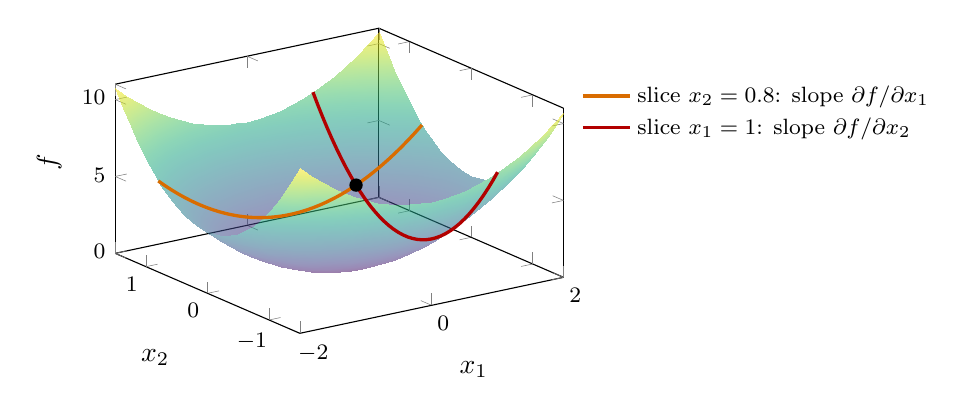
\begin{tikzpicture}
    \begin{axis}[
      width=0.6\textwidth, height=0.45\textwidth,
      view={-35}{30},
      xmin=-2, xmax=2, ymin=-1.5, ymax=1.5, zmin=0, zmax=11,
      xlabel={$x_1$}, ylabel={$x_2$}, zlabel={$f$},
      xtick={-2,0,2}, ytick={-1,0,1}, ztick={0,5,10},
      tick label style={font=\footnotesize},
      legend style={at={(1.02,0.85)}, anchor=north west, draw=none,
        font=\footnotesize},
      legend cell align=left,
    ]
      \addplot3[surf, shader=interp, colormap/viridis, opacity=0.55,
        domain=-2:2, y domain=-1.5:1.5, samples=25, forget plot]
        {x^2 + 3*y^2};
      \addplot3[very thick, orange!85!black, domain=-2:2, samples=40,
        samples y=0] ({x}, {0.8}, {x^2 + 1.92});
      \addlegendentry{slice $x_2 = 0.8$: slope $\partial f / \partial x_1$}
      \addplot3[very thick, red!70!black, domain=-1.5:1.5, samples=40,
        samples y=0] ({1}, {x}, {1 + 3*x^2});
      \addlegendentry{slice $x_1 = 1$: slope $\partial f / \partial x_2$}
      \addplot3[only marks, mark=*, mark size=2.2pt, black]
        coordinates {(1, 0.8, 2.92)};
    \end{axis}
  \end{tikzpicture}
  \caption{The surface $f(x_1, x_2) = x_1^2 + 3x_2^2$. Freezing one input
    cuts out a curve through the point $(1, 0.8)$ (black dot). The slopes
    of the two curves there are the partial derivatives
    $\partial f / \partial x_1 = 2$ and $\partial f / \partial x_2 = 4.8$.}
  \label{fig:ch02-slices}
\end{figure}

\subsection{The Gradient}
\label{sec:ch02-gradient}

Collect all the partial derivatives into one vector.

\begin{definition}[Gradient]
  \label{def:gradient}
  The \emph{gradient} of $f\colon \R^n \to \R$ at $\vect{x}$ is the vector
  of its partial derivatives:
  \[
    \nabla f(\vect{x}) =
    \left( \frac{\partial f}{\partial x_1}(\vect{x}), \dots,
           \frac{\partial f}{\partial x_n}(\vect{x}) \right).
  \]
\end{definition}

For $f(x_1, x_2) = x_1^2 + 3x_2^2$, the gradient is
$\nabla f(x_1, x_2) = (2x_1, 6x_2)$, and at $(1, 0.8)$ it is $(2, 4.8)$. The
gradient has one entry per input, so the gradient of a loss has exactly as
many entries as the model has parameters.

The gradient plays the role that $f'(x)$ played in one variable. The linear
approximation~\eqref{eq:ch02-linear-approx} becomes
\begin{equation}
  f(\vect{x} + \vect{h}) \approx f(\vect{x}) + \nabla f(\vect{x})^\top \vect{h}
  = f(\vect{x}) + \sum_{i=1}^n \frac{\partial f}{\partial x_i}(\vect{x})\, h_i ,
  \label{eq:ch02-linear-approx-n}
\end{equation}
for a small step $\vect{h}$: each coordinate contributes its own slope
times its own change. For example, from $(1, 0.8)$ the step
$\vect{h} = (0.1, -0.1)$ gives
$f \approx 2.92 + 2(0.1) + 4.8(-0.1) = 2.64$; the true value
$f(1.1, 0.7) = 2.68$ is close.

\paragraph{The direction of steepest ascent.}
Approximation~\eqref{eq:ch02-linear-approx-n} says how fast $f$ changes
when we move in any direction. Moving a small distance $t$ along a unit
vector $\vect{u}$ changes $f$ by about $t\, \nabla f(\vect{x})^\top
\vect{u}$, so the rate of change in direction $\vect{u}$ is
\[
  \nabla f(\vect{x})^\top \vect{u}
  = \|\nabla f(\vect{x})\| \cos \alpha ,
\]
where $\alpha$ is the angle between $\vect{u}$ and the gradient (the dot
product formula of \Cref{chap:ch03}). Since $\cos \alpha$ ranges from $-1$
to $1$, this gives the three facts that make the gradient useful.
\begin{itemize}
  \item $f$ increases fastest in the direction of $\nabla f(\vect{x})$
    ($\alpha = 0$), at rate $\|\nabla f(\vect{x})\|$.
  \item $f$ decreases fastest in the direction of $-\nabla f(\vect{x})$
    ($\alpha = \pi$).
  \item $f$ does not change, to first order, in directions perpendicular
    to the gradient ($\alpha = \pi / 2$). These are the directions along a
    \emph{level curve} $\{\vect{x} : f(\vect{x}) = c\}$, so the gradient is
    perpendicular to the level curves.
\end{itemize}
\Cref{fig:ch02-gradient} draws the level curves of
$x_1^2 + 3x_2^2$, which are ellipses, with gradient arrows crossing them at
right angles and pointing uphill. Gradient descent, the subject of
\Cref{sec:ch02-gd}, walks the opposite way.

\begin{figure}[ht]
  \centering
  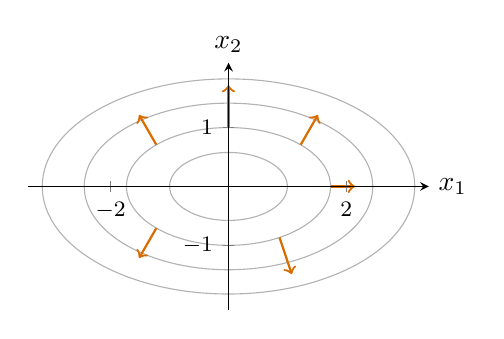
\begin{tikzpicture}
    \begin{axis}[
      width=0.55\textwidth,
      axis lines=middle, axis on top, axis equal image,
      xmin=-3.4, xmax=3.4, ymin=-2.1, ymax=2.1,
      xlabel={$x_1$}, ylabel={$x_2$},
      x label style={anchor=west}, y label style={anchor=south},
      xtick={-2,2}, ytick={-1,1},
      tick label style={font=\footnotesize},
    ]
      \draw[gray!60] (axis cs:0,0) ellipse [x radius=1, y radius=0.577];
      \draw[gray!60] (axis cs:0,0) ellipse [x radius=1.732, y radius=1];
      \draw[gray!60] (axis cs:0,0) ellipse [x radius=2.449, y radius=1.414];
      \draw[gray!60] (axis cs:0,0) ellipse [x radius=3.162, y radius=1.826];
      \foreach \px/\py/\gx/\gy in {
          1.732/0/0.416/0, 1.2247/0.7071/0.294/0.509,
          0/1/0/0.72, -1.2247/0.7071/-0.294/0.509,
          -1.2247/-0.7071/-0.294/-0.509, 0.866/-0.866/0.208/-0.624} {
        \edef\temp{\noexpand\draw[->, thick, orange!85!black]
          (axis cs:\px,\py) -- (axis cs:\px+\gx,\py+\gy);}
        \temp
      }
    \end{axis}
  \end{tikzpicture}
  \caption{Level curves (gray) of $f(x_1, x_2) = x_1^2 + 3x_2^2$, the
    ellipses $f = 1, 3, 6, 10$, with gradient arrows (orange) at points on
    the level curve $f = 3$. Each arrow is perpendicular to the curve and
    points uphill.}
  \label{fig:ch02-gradient}
\end{figure}

\subsection{In Code: Checking a Gradient}
\label{sec:ch02-gradient-code}

The central difference of \Cref{sec:ch02-numerical} extends to gradients
one coordinate at a time: nudge $x_j$ up and down by $h$, leave every other
coordinate fixed, and take the slope. Here we check the partial derivatives
of $g(x_1, x_2) = x_1^2 x_2 + e^{x_2}$ from \Cref{ex:ch02-partials} at the
point $(1, 0.5)$:

\begin{lstlisting}
import numpy as np

def g(x):
    return x[0]**2 * x[1] + np.exp(x[1])

def grad_g(x):                        # from Example 2.3
    return np.array([2 * x[0] * x[1], x[0]**2 + np.exp(x[1])])

def numerical_grad(f, x, h=1e-5):
    grad = np.zeros_like(x)
    for j in range(len(x)):
        e = np.zeros_like(x)
        e[j] = h                      # move only coordinate j
        grad[j] = (f(x + e) - f(x - e)) / (2 * h)
    return grad

x = np.array([1.0, 0.5])
grad_g(x)                             # [1.0, 2.6487]
numerical_grad(g, x)                  # [1.0, 2.6487]
np.abs(grad_g(x) - numerical_grad(g, x)).max()   # about 1e-11
\end{lstlisting}

The same function works for any $f\colon \R^n \to \R$, at the cost of two
evaluations of $f$ per coordinate.

\begin{aibox}
  In PyTorch, calling \texttt{loss.backward()} computes the gradient of the
  loss with respect to every parameter and stores it in each parameter's
  \texttt{.grad} field. An optimizer step is then exactly
  $\vect{w} \leftarrow \vect{w} - \eta \nabla L$, applied to every tensor of
  parameters at once. Unlike the loop above, \texttt{backward} does not
  nudge parameters one at a time: it applies the chain rule through the
  network and gets all the partial derivatives in a single pass.
\end{aibox}

\section{Gradient Descent}
\label{sec:ch02-gd}

At the bottom of a smooth valley the ground is flat, so a minimum of a
differentiable function is a point where the gradient is zero. For
$f(x) = x^2$ we can solve $f'(x) = 2x = 0$ by hand. For most functions,
including the loss of every neural network, the equation
$\nabla f(\vect{x}) = \vect{0}$ has no formula for its solution. Gradient
descent finds a minimum anyway, by starting somewhere and repeatedly
walking downhill.

\subsection{The Algorithm}
\label{sec:ch02-gd-algorithm}

To minimize a differentiable function $f\colon \R^n \to \R$:
\begin{enumerate}
  \item Choose a starting point $\vect{x}_0$, a \emph{step size} (or
    \emph{learning rate}) $\eta > 0$, and a tolerance $\varepsilon > 0$.
  \item For $k = 0, 1, 2, \dots$:
    \begin{enumerate}
      \item compute the gradient $\vect{g} = \nabla f(\vect{x}_k)$;
      \item if $\|\vect{g}\| < \varepsilon$, stop and return $\vect{x}_k$;
      \item otherwise step downhill: $\vect{x}_{k+1} = \vect{x}_k - \eta\,
        \vect{g}$.
    \end{enumerate}
\end{enumerate}

Each step moves in the direction of steepest descent,
$-\nabla f(\vect{x}_k)$ (\Cref{sec:ch02-gradient}). By the linear
approximation~\eqref{eq:ch02-linear-approx-n} with
$\vect{h} = -\eta \nabla f(\vect{x}_k)$,
\[
  f(\vect{x}_{k+1}) \approx f(\vect{x}_k) - \eta \, \|\nabla f(\vect{x}_k)\|^2 ,
\]
so for a small enough $\eta$ every step lowers $f$ until the gradient
vanishes. The step length is $\eta \|\nabla f(\vect{x}_k)\|$, so the steps
shorten automatically as the ground flattens near the minimum, even though
$\eta$ stays fixed. In practice, the loop also stops after a maximum number
of iterations, in case it never converges.

\subsection{A First Example}
\label{sec:ch02-gd-example}

Let $f(x) = (x - 3)^2 + 1$, whose minimum is $f(3) = 1$. Its derivative is
$f'(x) = 2(x - 3)$. Start at $x_0 = 0$ with $\eta = 0.25$. The update is
\[
  x_{k+1} = x_k - 0.25 \cdot 2(x_k - 3) = x_k - 0.5\,(x_k - 3),
\]
which can be rewritten as $x_{k+1} - 3 = 0.5\,(x_k - 3)$: each step halves
the distance to the minimum. \Cref{tab:ch02-gd-steps} lists the first
steps, and \Cref{fig:ch02-step-sizes}(a) draws them.

\begin{table}[ht]
  \centering
  \caption{Gradient descent on $f(x) = (x - 3)^2 + 1$ from $x_0 = 0$ with
    $\eta = 0.25$.}
  \label{tab:ch02-gd-steps}
  \begin{tabular}{@{}cccc@{}}
    \toprule
    $k$ & $x_k$ & $f(x_k)$ & $f'(x_k)$ \\
    \midrule
    $0$ & $0$ & $10$ & $-6$ \\
    $1$ & $1.5$ & $3.25$ & $-3$ \\
    $2$ & $2.25$ & $1.5625$ & $-1.5$ \\
    $3$ & $2.625$ & $1.1406$ & $-0.75$ \\
    $4$ & $2.8125$ & $1.0352$ & $-0.375$ \\
    $5$ & $2.9063$ & $1.0088$ & $-0.1875$ \\
    \bottomrule
  \end{tabular}
\end{table}

The derivative is negative at every step, meaning $f$ decreases to the
right, so each step moves right. As $x_k$ nears $3$ the derivative
shrinks and so do the steps. Reaching $|f'(x_k)| < 10^{-6}$ takes $23$
steps.

\subsection{Choosing the Step Size}
\label{sec:ch02-step-size}

The step size is the one number gradient descent asks us to choose, and it
matters a great deal. Repeating the computation above with a general
$\eta$ gives
\[
  x_{k+1} - 3 = (1 - 2\eta)(x_k - 3),
\]
so every step multiplies the distance to the minimum by $r = 1 - 2\eta$.
Four behaviors follow (\Cref{fig:ch02-step-sizes}(c)):
\begin{itemize}
  \item \emph{Too small} ($\eta = 0.05$, $r = 0.9$): steady but slow
    progress. After $20$ steps, $x \approx 2.64$.
  \item \emph{Well chosen} ($\eta = 0.25$, $r = 0.5$): fast, steady
    convergence.
  \item \emph{Large} ($\eta = 0.9$, $r = -0.8$): every step overshoots the
    minimum and lands on the other side, but a little closer. The iterates
    zig-zag inward (\Cref{fig:ch02-step-sizes}(b)).
  \item \emph{Too large} ($\eta = 1.05$, $r = -1.1$): every step overshoots
    by more than it gained, and the iterates fly off to infinity. Gradient
    descent \emph{diverges}.
\end{itemize}
Here gradient descent converges exactly when $|1 - 2\eta| < 1$, that is,
$0 < \eta < 1$. A steeper function needs a smaller step: for
$f(x) = c\,(x - 3)^2$ the factor is $1 - 2c\eta$, so the safe range
shrinks to $\eta < 1/c$.

\begin{figure}[ht]
  \centering
  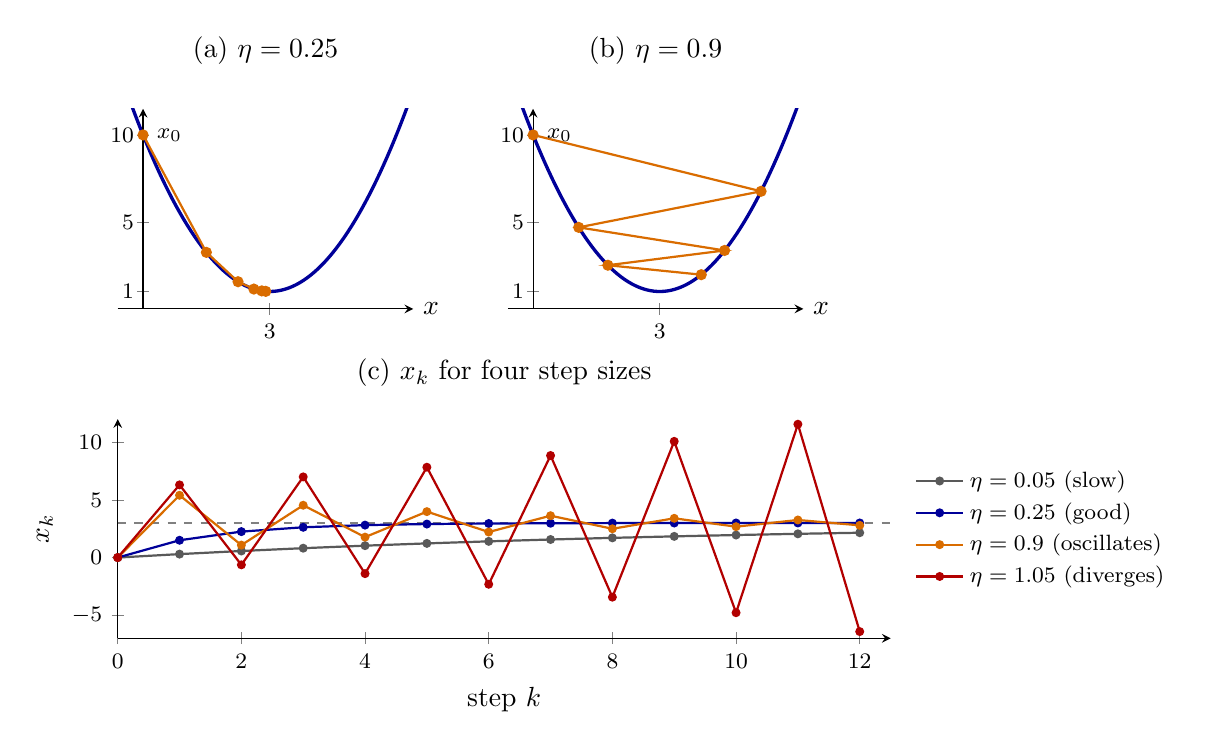
\begin{tikzpicture}
    \pgfplotsset{
      par/.style={
        width=0.44\textwidth, height=0.34\textwidth,
        axis lines=middle, axis on top,
        xmin=-0.6, xmax=6.4, ymin=0, ymax=11.5,
        xtick={3}, ytick={1,5,10},
        xlabel={$x$}, x label style={anchor=west},
        title style={yshift=1.5ex},
        tick label style={font=\footnotesize},
        yticklabel style={fill=white, inner sep=1pt},
      },
      path/.style={thick, orange!85!black, mark=*, mark size=1.6pt},
    }
    \begin{axis}[par, name=good, title={(a) $\eta = 0.25$}]
      \addplot[very thick, blue!60!black, domain=-0.5:6.3, samples=80]
        {(x-3)^2 + 1};
      \addplot[path] coordinates {(0,10) (1.5,3.25) (2.25,1.5625)
        (2.625,1.1406) (2.8125,1.0352) (2.9062,1.0088)};
      \node[anchor=west, font=\footnotesize] at (axis cs:0.1,10) {$x_0$};
    \end{axis}
    \begin{axis}[par, name=big, at={(good.east)}, anchor=west, xshift=1.2cm,
        title={(b) $\eta = 0.9$}]
      \addplot[very thick, blue!60!black, domain=-0.5:6.3, samples=80]
        {(x-3)^2 + 1};
      \addplot[path] coordinates {(0,10) (5.4,6.76) (1.08,4.6864)
        (4.536,3.3593) (1.7712,2.5099) (3.983,1.9664)};
      \node[anchor=west, font=\footnotesize] at (axis cs:0.1,10) {$x_0$};
    \end{axis}
    \begin{axis}[
      at={(good.south west)}, anchor=north west, yshift=-1.4cm,
      width=0.94\textwidth, height=0.36\textwidth,
      axis lines=left, xmin=0, xmax=12.5, ymin=-7, ymax=12,
      xtick={0,2,...,12}, ytick={-5,0,5,10},
      xlabel={step $k$}, ylabel={$x_k$},
      tick label style={font=\footnotesize},
      title={(c) $x_k$ for four step sizes},
      title style={yshift=0.5ex},
      legend style={at={(1.02,0.5)}, anchor=west, draw=none,
        font=\footnotesize},
      legend cell align=left,
    ]
      \addplot[dashed, gray, domain=0:12.5, forget plot] {3};
      \addplot[thick, gray!70!black, mark=*, mark size=1.2pt] coordinates {
        (0,0) (1,0.3) (2,0.57) (3,0.813) (4,1.0317) (5,1.2285) (6,1.4057)
        (7,1.5651) (8,1.7086) (9,1.8377) (10,1.954) (11,2.0586) (12,2.1527)};
      \addlegendentry{$\eta = 0.05$ (slow)}
      \addplot[thick, blue!60!black, mark=*, mark size=1.2pt] coordinates {
        (0,0) (1,1.5) (2,2.25) (3,2.625) (4,2.8125) (5,2.9062) (6,2.9531)
        (7,2.9766) (8,2.9883) (9,2.9941) (10,2.9971) (11,2.9985) (12,2.9993)};
      \addlegendentry{$\eta = 0.25$ (good)}
      \addplot[thick, orange!85!black, mark=*, mark size=1.2pt] coordinates {
        (0,0) (1,5.4) (2,1.08) (3,4.536) (4,1.7712) (5,3.983) (6,2.2136)
        (7,3.6291) (8,2.4967) (9,3.4027) (10,2.6779) (11,3.2577) (12,2.7938)};
      \addlegendentry{$\eta = 0.9$ (oscillates)}
      \addplot[thick, red!70!black, mark=*, mark size=1.2pt] coordinates {
        (0,0) (1,6.3) (2,-0.63) (3,6.993) (4,-1.3923) (5,7.8315) (6,-2.3147)
        (7,8.8462) (8,-3.4308) (9,10.0738) (10,-4.7812) (11,11.5594)
        (12,-6.4153)};
      \addlegendentry{$\eta = 1.05$ (diverges)}
    \end{axis}
  \end{tikzpicture}
  \caption{Gradient descent on $f(x) = (x - 3)^2 + 1$ from $x_0 = 0$.
    (a) With $\eta = 0.25$, the iterates (orange) slide down to the minimum
    at $x = 3$. (b) With $\eta = 0.9$, each step overshoots to the other
    side, but the iterates still close in. (c) The iterates $x_k$ for four
    step sizes; the dashed line is the minimizer $x = 3$.}
  \label{fig:ch02-step-sizes}
\end{figure}

In practice we cannot compute the safe range, because we do not know how
steep the loss is everywhere. The usual approach is to try step sizes a
factor of ten apart, such as $10^{-1}$, $10^{-2}$, and $10^{-3}$, and
watch the value of $f$: if it rises or becomes \texttt{nan}, the step is too
large; if it falls very slowly, the step is too small.

\subsection{Gradient Descent in Several Variables}
\label{sec:ch02-gd-multi}

Nothing changes in the algorithm when there are many variables, but a new
difficulty appears. Take $f(x_1, x_2) = x_1^2 + 3x_2^2$, with gradient
$(2x_1, 6x_2)$ and minimum at the origin. The update acts on each
coordinate separately:
\[
  x_1 \leftarrow (1 - 2\eta)\, x_1, \qquad
  x_2 \leftarrow (1 - 6\eta)\, x_2 .
\]
Each coordinate has its own factor, as if we were running two
one-variable problems with one shared step size. Both converge only if
$|1 - 2\eta| < 1$ and $|1 - 6\eta| < 1$, which requires $\eta < 1/3$. The
steepest direction sets the limit on the step size, and the flattest
direction then determines how slowly we converge.

\Cref{fig:ch02-gd-paths} shows two runs from $(-2.5, 1.2)$. With
$\eta = 0.1$ the factors are $0.8$ and $0.4$: $x_2$ collapses quickly and
the path then creeps along the flat $x_1$ direction. With $\eta = 0.25$
the factors are $0.5$ and $-0.5$: both coordinates halve each step, but
$x_2$ flips sign every time and the path zig-zags across the valley. At
$\eta = 0.35$, which would be a fine step for $x_1$ alone, the $x_2$
factor is $-1.1$ and the iteration diverges. When a loss is much steeper
in some directions than in others, plain gradient descent is forced into
this trade-off. Momentum and Adam (\Cref{chap:ch08}) are designed to
escape it.

\begin{figure}[ht]
  \centering
  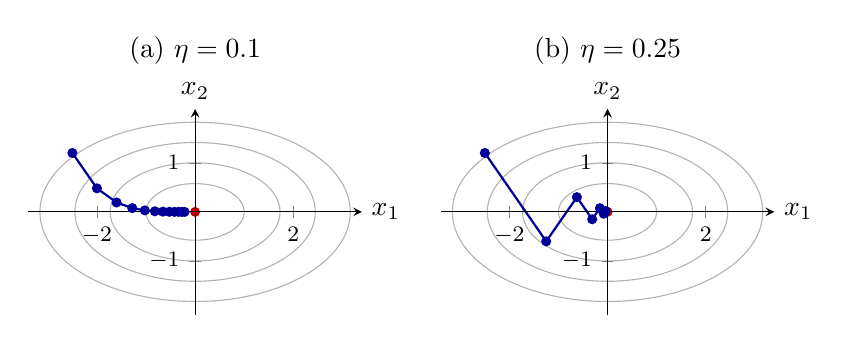
\begin{tikzpicture}
    \pgfplotsset{
      lvl/.style={
        width=0.48\textwidth,
        axis lines=middle, axis on top, axis equal image,
        xmin=-3.4, xmax=3.4, ymin=-2.1, ymax=2.1,
        xlabel={$x_1$}, ylabel={$x_2$},
        x label style={anchor=west}, y label style={anchor=south},
        xtick={-2,2}, ytick={-1,1},
        title style={yshift=1.5ex},
        tick label style={font=\footnotesize},
      },
    }
    \begin{axis}[lvl, name=slow, title={(a) $\eta = 0.1$}]
      \draw[gray!60] (axis cs:0,0) ellipse [x radius=1, y radius=0.577];
      \draw[gray!60] (axis cs:0,0) ellipse [x radius=1.732, y radius=1];
      \draw[gray!60] (axis cs:0,0) ellipse [x radius=2.449, y radius=1.414];
      \draw[gray!60] (axis cs:0,0) ellipse [x radius=3.162, y radius=1.826];
      \addplot[thick, blue!60!black, mark=*, mark size=1.4pt]
        coordinates {(-2.5,1.2) (-2,0.48) (-1.6,0.192) (-1.28,0.0768)
          (-1.024,0.0307) (-0.8192,0.0123) (-0.6554,0.0049)
          (-0.5243,0.002) (-0.4194,0.0008) (-0.3355,0.0003)
          (-0.2684,0.0001) (-0.2147,0.0001)};
      \fill[red!70!black] (axis cs:0,0) circle (1.8pt);
    \end{axis}
    \begin{axis}[lvl, at={(slow.east)}, anchor=west, xshift=1cm,
        title={(b) $\eta = 0.25$}]
      \draw[gray!60] (axis cs:0,0) ellipse [x radius=1, y radius=0.577];
      \draw[gray!60] (axis cs:0,0) ellipse [x radius=1.732, y radius=1];
      \draw[gray!60] (axis cs:0,0) ellipse [x radius=2.449, y radius=1.414];
      \draw[gray!60] (axis cs:0,0) ellipse [x radius=3.162, y radius=1.826];
      \addplot[thick, blue!60!black, mark=*, mark size=1.4pt]
        coordinates {(-2.5,1.2) (-1.25,-0.6) (-0.625,0.3) (-0.3125,-0.15)
          (-0.15625,0.075) (-0.078125,-0.0375) (-0.0390625,0.01875)};
      \fill[red!70!black] (axis cs:0,0) circle (1.8pt);
    \end{axis}
  \end{tikzpicture}
  \caption{Gradient descent on $f(x_1, x_2) = x_1^2 + 3x_2^2$ from
    $(-2.5, 1.2)$, drawn over its level curves. (a) A small step settles
    the steep $x_2$ direction at once, then creeps along the flat $x_1$
    direction. (b) A larger step converges faster but zig-zags across the
    steep direction. The minimum is marked in red.}
  \label{fig:ch02-gd-paths}
\end{figure}

\subsection{What Gradient Descent Finds}
\label{sec:ch02-gd-finds}

Gradient descent stops where the gradient is zero. Such a point is called
a \emph{stationary point}, and there are three kinds.
\begin{itemize}
  \item A \emph{minimum}, which is what we want.
  \item A \emph{maximum}. Gradient descent essentially never stops here:
    every nearby point is lower, so any step away from the top runs
    downhill.
  \item A \emph{saddle point}, where $f$ curves up in some directions and
    down in others. For $f(x_1, x_2) = x_1^2 - x_2^2$, the origin is
    a minimum along $x_1$ but a maximum along $x_2$. Started from $(1, 0)$,
    gradient descent never moves $x_2$ and converges to the saddle.
    Started from $(1, 10^{-6})$, the tiny $x_2$ grows by a factor of
    $1 + 2\eta$ every step and the iterates escape downhill.
\end{itemize}
Saddle points are therefore unstable, and a little noise is enough to leave
them. Local minima are not: as \Cref{sec:ch01-local-global} showed, a
non-convex function can trap gradient descent in a valley that is not the
lowest one, and which valley it reaches depends on the starting point.

For convex functions none of these problems arise. A convex
differentiable function has no maxima or saddle points to stop at, and by
\Cref{thm:ch01-local-global} its local minima are global. With a small
enough step size, gradient descent on a convex function approaches the
global minimum from any starting point.

\subsection{In Code: Minimizing Functions}
\label{sec:ch02-gd-code}

The algorithm of \Cref{sec:ch02-gd-algorithm} fits in a few lines. The
function takes the gradient as a Python function, so the same code
minimizes any differentiable $f$ whose gradient we can write down:

\begin{lstlisting}
import numpy as np

def gradient_descent(grad, x0, lr, tol=1e-6, max_iters=10_000):
    x = np.array(x0, dtype=float)
    for k in range(max_iters):
        g = grad(x)
        if np.linalg.norm(g) < tol:     # flat enough: done
            return x, k
        x = x - lr * g                  # step downhill
    return x, max_iters
\end{lstlisting}

\paragraph{One variable.}
The example of \Cref{sec:ch02-gd-example} reproduces the $23$ steps
found there:

\begin{lstlisting}
grad = lambda x: 2 * (x - 3)            # f(x) = (x - 3)^2 + 1
gradient_descent(grad, [0.0], lr=0.25)  # x = 2.9999996, after 23 steps
\end{lstlisting}

\paragraph{Comparing step sizes.}
Setting \texttt{tol=0} turns off the stopping test, so the loop runs
exactly \texttt{max\_iters} steps. After $20$ steps, the four step sizes of
\Cref{sec:ch02-step-size} give:

\begin{lstlisting}
for lr in [0.05, 0.25, 0.9, 1.05]:
    x, _ = gradient_descent(grad, [0.0], lr, tol=0, max_iters=20)
    print(lr, x)
# 0.05  [2.635]       too small: still far from 3
# 0.25  [2.999997]    good
# 0.9   [2.965]       oscillating, but closing in
# 1.05  [-17.18]      diverging
\end{lstlisting}

\paragraph{Two variables.}
On the bowl $x_1^2 + 3x_2^2$ of \Cref{sec:ch02-gd-multi}, the step size
must stay below $1/3$:

\begin{lstlisting}
grad = lambda x: np.array([2 * x[0], 6 * x[1]])

gradient_descent(grad, [-2.5, 1.2], lr=0.1)    # ~[0, 0] after 70 steps
gradient_descent(grad, [-2.5, 1.2], lr=0.25)   # ~[0, 0] after 24 steps
gradient_descent(grad, [-2.5, 1.2], lr=0.35, max_iters=50)
                                               # x2 = 140.9: diverged
\end{lstlisting}

\paragraph{A narrow, curved valley.}
Real loss functions are rarely tidy bowls. A standard test is the
\emph{Rosenbrock function}, here in the form
\[
  f(x_1, x_2) = (1 - x_1)^2 + 10\,(x_2 - x_1^2)^2 ,
\]
whose minimum $f = 0$ lies at $(1, 1)$ at the bottom of a curved valley
with steep walls. Its gradient follows from the rules of
\Cref{sec:ch02-rules}:

\begin{lstlisting}
def rosenbrock_grad(x):
    dx1 = -2 * (1 - x[0]) - 40 * x[0] * (x[1] - x[0]**2)
    dx2 = 20 * (x[1] - x[0]**2)
    return np.array([dx1, dx2])

gradient_descent(rosenbrock_grad, [-1.0, 1.0], lr=0.01)
# ~[1, 1] after 3241 steps
\end{lstlisting}

The bowl took $24$ steps; this valley takes over $3000$. The steep walls
force a small step size, and with that step, progress along the gently
sloping valley floor is slow. This is the multi-variable trade-off of
\Cref{sec:ch02-gd-multi} in a harder form, and it is the everyday
situation when training neural networks.

\begin{aibox}
  Training a neural network is gradient descent on its loss, with two
  changes. The gradient is computed by backpropagation instead of by
  hand, and it is estimated from a small random batch of
  training examples rather than the whole dataset, which makes each step
  cheap but noisy. This \emph{stochastic gradient descent} and its
  refinements, momentum and Adam, are the subject of \Cref{chap:ch08}. The
  learning rate remains the most important setting to tune, for exactly
  the reasons shown in \Cref{fig:ch02-step-sizes}.
\end{aibox}

\section{Summary}
\label{sec:ch02-summary}

\begin{itemize}
  \item The \emph{derivative} $f'(x) = \lim_{h \to 0} \bigl(f(x + h) -
    f(x)\bigr)/h$ is the slope of the graph at $x$. Near $x$, a
    differentiable function is approximately a line:
    $f(x + h) \approx f(x) + f'(x)\, h$.
  \item Derivatives are computed from a short table of basic functions and
    the sum, product, quotient, and chain rules. The sigmoid satisfies
    $\sigma' = \sigma(1 - \sigma)$, which is at most $\tfrac14$ and nearly
    zero for large inputs.
  \item Derivatives fail at corners, such as ReLU at $0$, and at jumps, such
    as the sign function. Frameworks pick a value at a corner; a jump or
    a flat function gives gradient descent nothing to follow.
  \item A \emph{partial derivative} $\partial f / \partial x_i$ varies one
    input and holds the others fixed. The \emph{gradient} $\nabla f$
    collects all of them, has one entry per input, and points in the
    direction of steepest ascent, perpendicular to the level curves.
  \item The central difference $\bigl(f(x + h) - f(x - h)\bigr)/(2h)$
    approximates a derivative without calculus; comparing it with a
    formula is a \emph{gradient check}.
  \item \emph{Gradient descent} minimizes $f$ by repeating
    $\vect{x} \leftarrow \vect{x} - \eta \nabla f(\vect{x})$ until the
    gradient is nearly zero. Each small step lowers $f$ by about
    $\eta \|\nabla f\|^2$.
  \item The step size $\eta$ decides everything: too small is slow, too
    large oscillates or diverges. With several variables, the steepest
    direction limits $\eta$ and the flattest direction limits the speed.
  \item Gradient descent stops at stationary points. It escapes maxima and
    saddle points easily but can be trapped in a local minimum; for convex
    functions, it reaches the global minimum.
\end{itemize}
